\documentclass[11pt]{article}
\usepackage[letterpaper,margin=1in]{geometry}
\usepackage{color}
\usepackage[dvipdfmx]{graphicx}
\usepackage{amsbsy}
\usepackage{amsmath}
\usepackage{adjustbox}
\usepackage{url}

\newcommand{\argmax}{\mathop{\rm arg~max}\limits}

\begin{document}
\title{Analysis Report on Assignment 1: K-nearest neighbors}
\author{Yoshinari Fujinuma}
\date{}
\maketitle

%\section{What is the relationship between the number of training examples and accuracy?}
\section{The relationship between the number of training examples, $k$, and accuracy?}
The following two graph shows the relationship between training examples and accuracy:
\begin{figure}[htb]
  \begin{center}
   \begin{tabular}{c}

    \begin{minipage}{0.5\hsize}
     \begin{center}
     \scalebox{0.33}
      {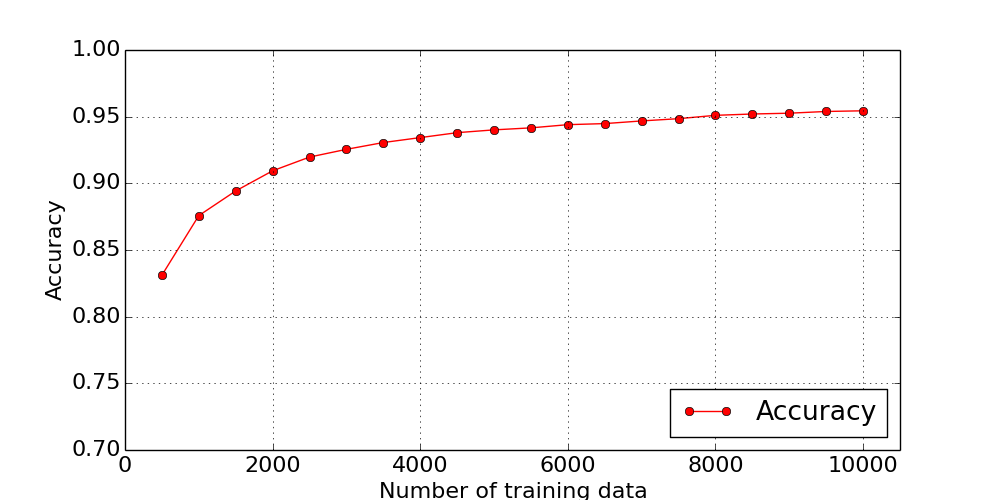
\includegraphics[]{figure_1.png}}
   
      \caption{The relationship between the number of training examples and accuracy. The value of $k$ is fixed to $3$. }
      \label{fig:corpus_size}
     \end{center}
    \end{minipage}

    \begin{minipage}{0.01\hsize}
    \end{minipage}

    \begin{minipage}{0.5\hsize}
     \begin{center}
      \scalebox{0.33}
      {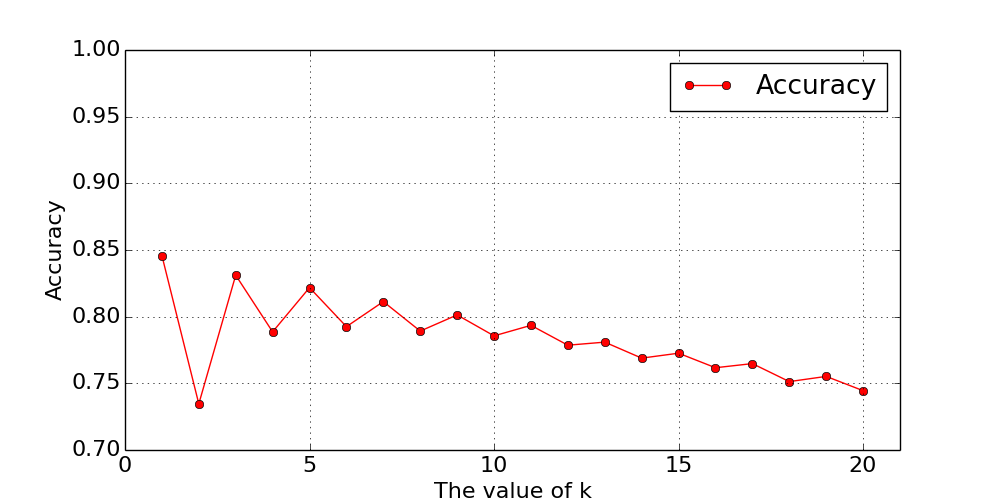
\includegraphics[]{figure_2.png}}
      \caption{The relationship between $k$ and accuracy.}
     \end{center}
    \end{minipage}

  \end{tabular}
 \end{center}
\end{figure}

As the number of training examples increases, the higher the accuracy becomes.

%\section{What is the relationship between $k$ and accuracy?}
%The following graph shows the relationship between $k$ and accuracy:
%\begin{figure}[htb]
%  %\begin{minipage}{0.5\hsize}
%   \begin{center}
%    \scalebox{0.4}
%     {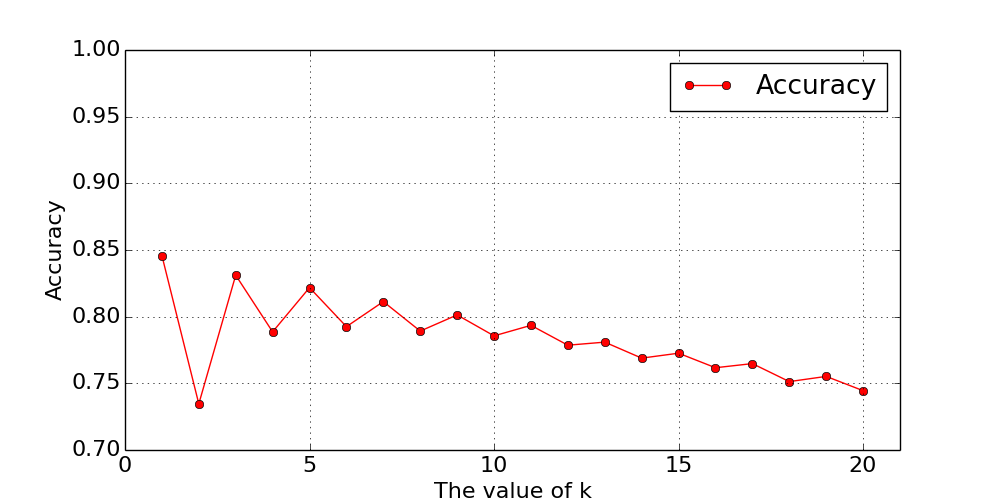
\includegraphics[]{figure_2.png}}
%    \end{center}
%    \caption{The relationship between $k$ and accuracy.}
%    \label{fig:corpus_size}
%  %\end{minipage}
%%\vspace{0.1cm}
%\end{figure}

\section{What numbers get confused with each other most easily?}

\end{document}

